\documentclass[11pt, oneside]{article}   	% use "amsart" instead of "article" for AMSLaTeX format


% \usepackage{draftwatermark}
% \SetWatermarkText{Draft}
% \SetWatermarkScale{5}
% \SetWatermarkLightness {0.9} 
% \SetWatermarkColor[rgb]{0.7,0,0}


\usepackage{geometry}                		% See geometry.pdf to learn the layout options. There are lots.
\geometry{letterpaper}                   		% ... or a4paper or a5paper or ... 
%\geometry{landscape}                		% Activate for for rotated page geometryhttps://www.washingtonpost.com/world/europe/amid-impeachment-probe-gordon-sondland-is-overseeing-a-renovation-of-his-residence-that-has-cost-1-million-in-taxpayer-money/2019/10/16/d0eece92-ef86-11e9-bb7e-d2026ee0c199_story.html?tid=sm_tw
%\usepackage[parfill]{parskip}    		% Activate to begin paragraphs with an empty line rather than an indent
\usepackage{graphicx}				% Use pdf, png, jpg, or eps� with pdflatex; use eps in DVI mode
								% TeX will automatically convert eps --> pdf in pdflat						\label{thm:integral_domain}

								% TeX will automatically convert eps --> pdf in pdflatex		
\usepackage{amssymb}
\usepackage{amsmath}
\usepackage{amsthm}
\usepackage{mathrsfs}
\usepackage[hyphens,spaces,obeyspaces]{url}
\usepackage{url}
\usepackage{hyperref}
\usepackage{subcaption}
\usepackage{authblk}
\usepackage{mathtools}
\usepackage{graphicx}
\usepackage[export]{adjustbox}
\usepackage{fixltx2e}
\usepackage{hyperref}
\usepackage{alltt}
\usepackage{color}
\usepackage[utf8]{inputenc}
\usepackage[english]{babel}
\usepackage{float}
\usepackage{bigints}
\usepackage{braket}
\usepackage{siunitx}
\usepackage{mathtools}
\usepackage[most]{tcolorbox}



\usepackage[hyphenbreaks]{breakurl}

\newtheorem{thm}{Theorem}[section]
% \newtheorem{defn}[thm]{Definition}
\theoremstyle{definition}
\newtheorem{definition}{Definition}[section]
\newtheorem{proposition}{Proposition}[section]
\newtheorem{lemma}{Lemma}[section]
\newtheorem{example}{Example}[section]




\newcommand{\veq}{\mathrel{\rotatebox{90}{$=$}}}
\DeclareMathOperator{\bda}{\Big \downarrow}


\DeclareMathOperator{\E}{\mathbb{E}}
\newcommand{\argmax}{\operatornamewithlimits{argmax}}
\newcommand{\argmin}{\operatornamewithlimits{argmin}}

\title{How Did Price's Metonic Cycle Gear Train Work?}
\author{David Meyer \\ dmm@\{1-4-5.net,uoregon.edu\}}

\date{Last update: March 23, 2021}							% Activate to display a given date or no date



\begin{document}
\maketitle

\section{Introduction}
The advent of new insight into the structure and function of the Antikythera Mechanism \cite{Freeth2021} made me wonder exactly how 
Derek J. de Solla Price's \cite{wiki:price} proposed Metonic Cycle gear train in the Mechanism works. I decided to look at the Metonic gear 
train first since it is a simple gear train;  specifically this gear train has no epicyclic gears \cite{Wright2005} or pin-and-slot devices \cite{pin_and_slot_device,Evans2010}.

\bigskip
\noindent
I'll just note here that while Price's Metonic Cycle gear train is generally considered to be correct \cite{Freeth2006}, his interpretation of its output
(and hence the upper dial on the back of the Mechanism) as well as how the Metonic Cycle pointer was turned, is considered
to be wrong \cite{challenging_the_classic_research}.

\bigskip
\noindent
These notes briefly investigate how and why Price's Metonic Cycle gear train works.

\section{First, What Is The Metonic Cycle?}
The Metonic Cycle is \emph{a period of approximately nineteen years after which the phases of the moon recur on the same day of the year}. It is defined by 
observation to be 235 synodic (lunar) months,  just 1h27m33s longer than nineteen tropical years. Learning from the Babylonian and Hebrew lunisolar calendars 
in which the years 3, 6, 8, 11, 14, 17, and 19 are the long (13-month) years, the $5^{th} \text{century BC}$ Greek mathematician, 
astronomer, geometer, and engineer Meton of Athens \cite{wiki:menton} judged the cycle to be a whole number of days, specifically 6,940 days. Using these integer 
values facilitated  the construction of a lunisolar calendar.

\bigskip
\noindent
One Metonic Cycle is defined to be 19 tropical years, which is 235 synodic months (lunar phases), which in turn equals 6,939.688 days. Since
19 tropical years equals 6,939.602 days the difference of  $6,939.688 - 6,939.602 = 0.086$ days/cycle means that after twelve cycles there 
will be a 1.032 day difference between observation and calculation (since $0.086 \text{ days/cycle} * 12 \text{ cycles} = 
1.032 \text{ days}$).  

\bigskip
\noindent
The Metonic Cycle also turns out to be very close to integer multiples of two other important lunar periods:

\bigskip
\begin{itemize}
  \item 254 sidereal months (lunar orbits) = 6,939.702 days
  \item 255 draconic months (lunar nodes) = 6,939.116 days
\end{itemize}

\bigskip
\noindent
So in  summary: 

\begin{flushleft}
\begin{tabular}{@{}l@{\ }l@{\qquad}l}
  One Metonic Cycle
  & = 19 tropical years                            & \# 6,939.602 days \\
  & $\approx$ 235 synodic months        & \# 6,939.688 days \\
  & $\approx$ 254 sidereal months        & \# 6,939.702 days \\
  & $\approx$ 255 draconic months       & \# 6,939.116 days \\
\end{tabular}
\end{flushleft}


% \begin{equation*}
% \begin{array}{lllll}
%   \text{One Metonic Cycle}
%   &=& \text{19 tropical years}                     &\qquad  \mathrel{\#} \text {6,939.602 days}    \\
%   &\approx& \text {235 synodic months}    &\qquad  \mathrel{\#} \text{6,939.688 days}      \\
%   &\approx& \text {254 sidereal months}    &\qquad  \mathrel{\#} \text {6,939.702 days}     \\
%   &\approx& \text {255 draconic months}   &\qquad  \mathrel{\#} \text {6,939.116 days}     \\
% \end{array}
% \end{equation*}


\bigskip
\noindent
Interestingly $\frac{254}{19} \approx 13.36842$,  which is said to be an important astronomical constant.\footnote{Why exactly this 
constant is considered to be "important" is something I have not been able to learn.}

\bigskip
\bigskip
\begin{figure}[H]
  \center{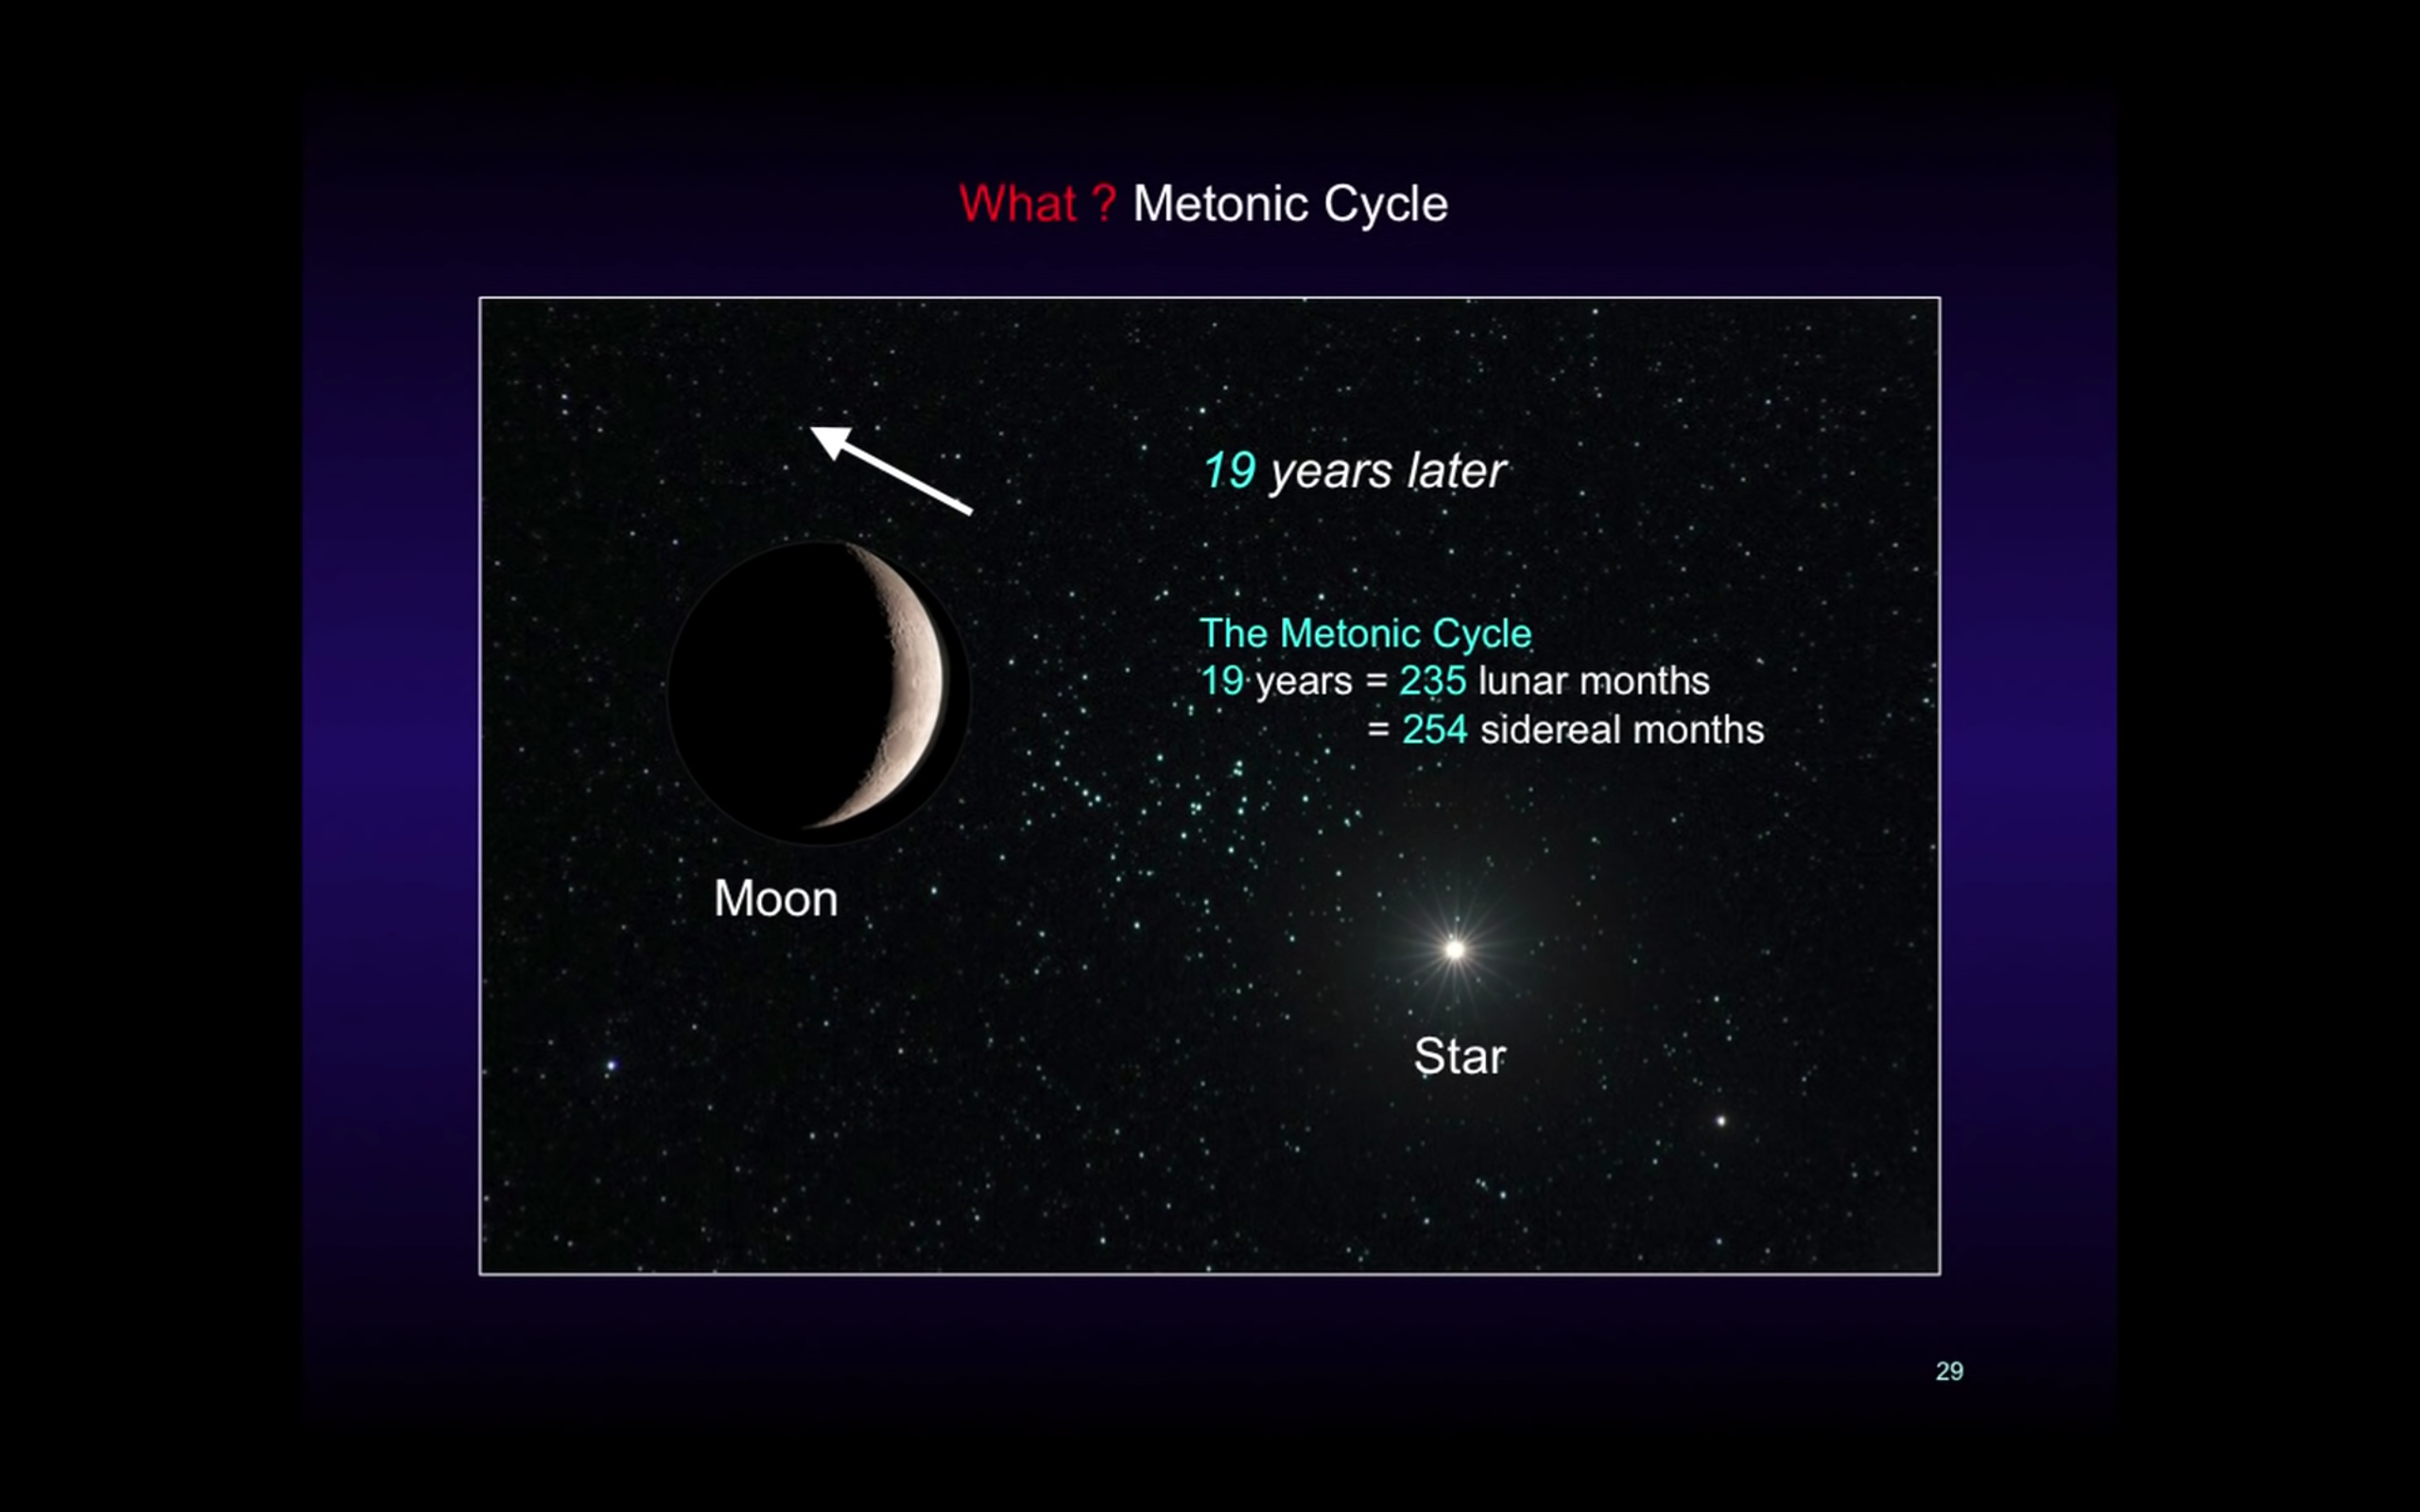
\includegraphics[scale=0.25,cfbox=red] {images/metonic.png}}
  \caption{The Metonic Cycle \cite{youtube:freeth2021}}
  \label{fig:metonic_cycle}
\end{figure}

\bigskip
\bigskip
\noindent
This is all very interesting. However, the Metonic Cycle seems to be a coincidence. The periods of the Moon's orbit around the Earth and the Earth's 
orbit around the Sun are believed to be independent, and not to have any known physical resonance. An example of a non-coincidental 
cycle is the orbit of Mercury, with its 3:2 spin-orbit resonance \cite{Correia2004}. 

\section{Price's Metonic Cycle Gearing Scheme}
Price's Metonic gearing scheme, described in his classic work "Gears from the Greeks. The Antikythera Mechanism: A Calendar Computer from 
ca. 80 B. C. T" \cite{gears_from_the_greeks},  is shown in Figure \ref{fig:general_gearing_plan}. As we will see below, Price's Metonic Cycle gear 
train essentially calculates the average position of the Moon in the Zodiac.

\bigskip
\begin{figure}[H]
\center{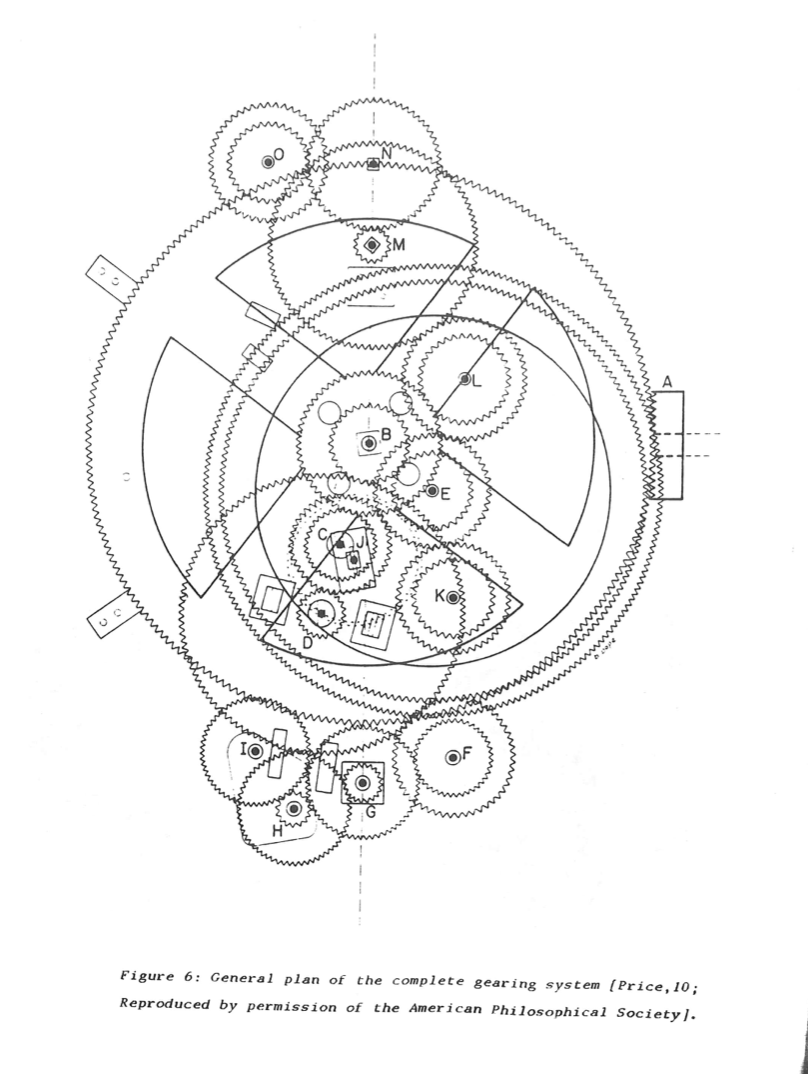
\includegraphics[scale=0.65,frame] {images/general_gearing_plan.png}}
\caption{Price's General Gearing Plan \cite{gears_from_the_greeks}}
\label{fig:general_gearing_plan}
\end{figure}

\bigskip
\noindent
For calculating gear ratios,  Price's sectional gearing diagram is more useful. As we can see from Figure \ref{fig:sectional_gearing}, the gears of interest
are b2, c1, c2, d1, d2, and e2, with the following tooth counts\footnote{Price argued with Greek physicist Charalambos Karakalos about 
tooth counts on various gears \cite{youtube:freeth2021}.}:

\bigskip
\begin{figure}[H]
  \center{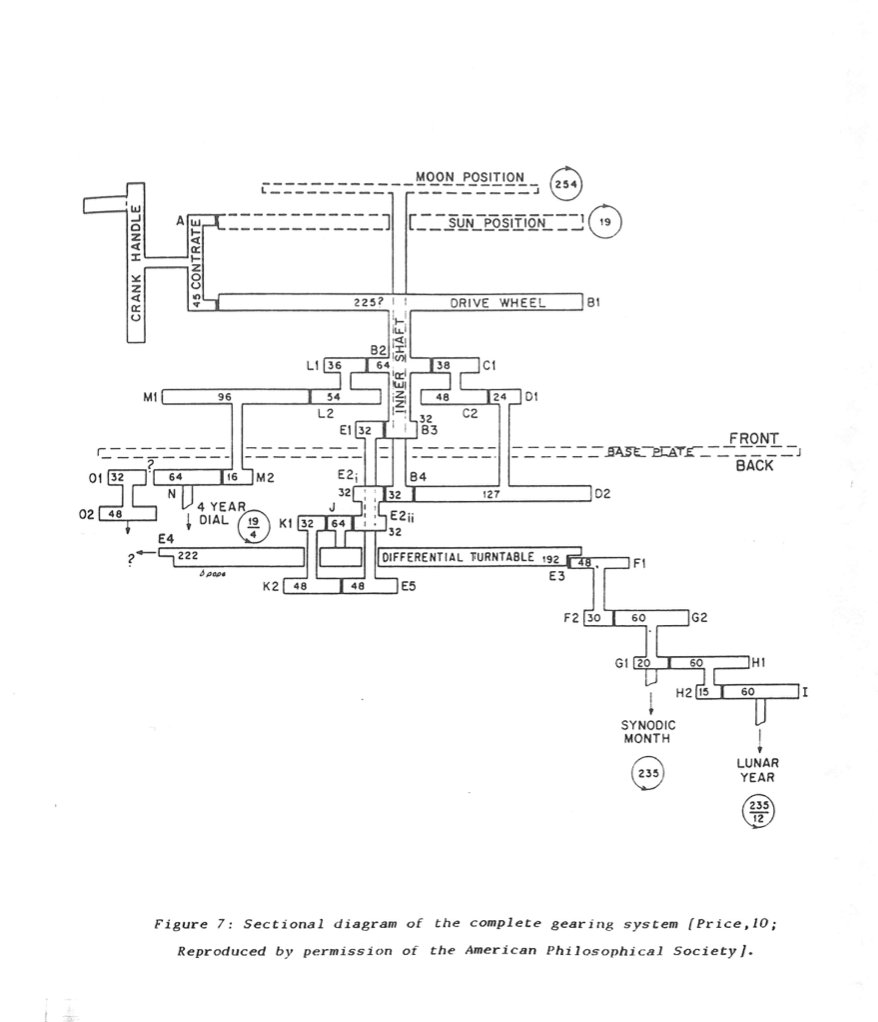
\includegraphics[scale=0.50,frame] {images/sectional_diagram.png}}
  \caption{Price's Sectional Gearing Diagram \cite{gears_from_the_greeks}}
  \label{fig:sectional_gearing}
\end{figure}
\bigskip
\bigskip
\bigskip
\begin{minipage}[c]{0.45\textwidth}
  \begin{itemize}
    \item b2: 64 teeth
    \item c1: 38 teeth
    \item c2: 48 teeth
    \item d1: 24 teeth
    \item d2: 127 teeth
    \item e2: 32 teeth
  \end{itemize}
\end{minipage}
\hfill
\begin{minipage}[c]{0.5\textwidth}
  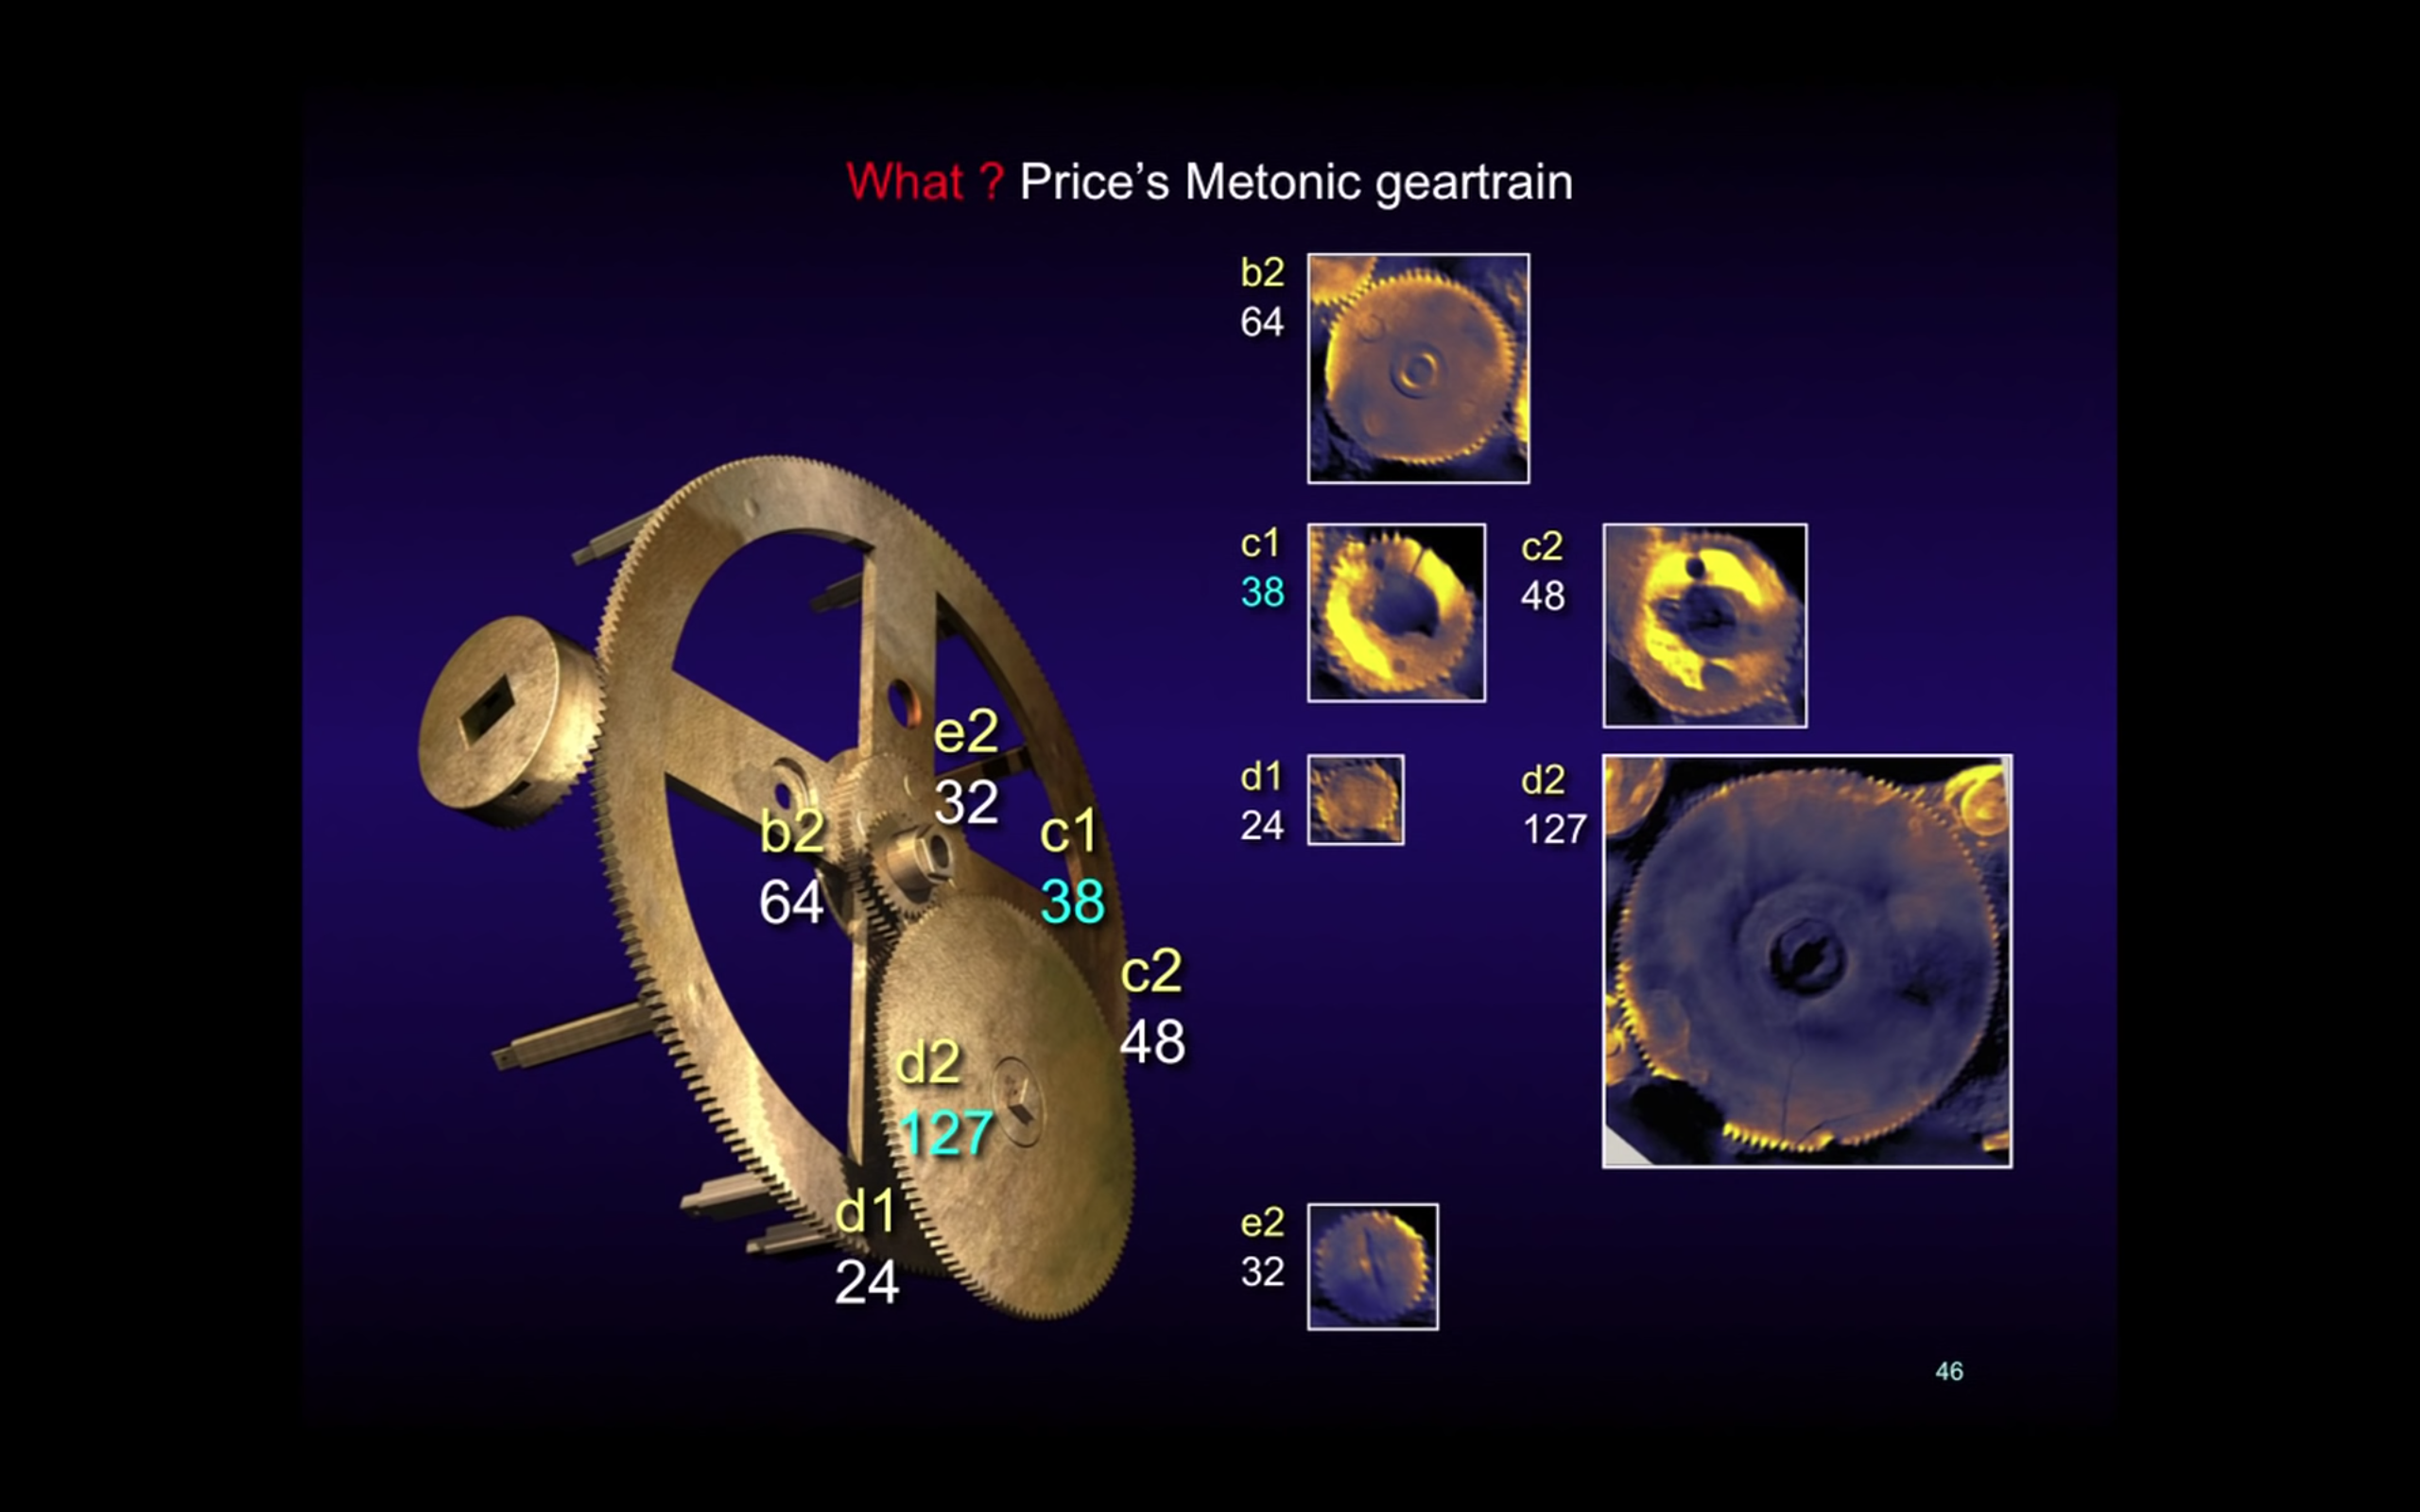
\includegraphics[width=\textwidth,cfbox=red]{images/price_metonic_gear_train.png}
  \captionof{figure}{The Metonic Gear Train \cite{youtube:freeth2021}}
\end{minipage}

\noindent
We know that in simple gear trains we can calculate the Gear Ratio (GR) as 

\bigskip
\begin{center}
{\Large $\text{GR} = \frac{\text{Number of Teeth on the Driven Gear}}{\text{Number of Teeth on the Driver Gear}}$}
\end{center}

\bigskip
\noindent
and we know that the driven gear rotates in the opposite direction of the driver gear. 


\bigskip
\noindent
With this information we can start to calculate what Price's Metonic gear train does. 

\bigskip
\noindent
Specifically:

\begin{equation*}
\begin{array}{lllll}
\frac{\text{b2}}{\text{c1}} &= - \frac{64}{38} = - \frac{32}{19} & \quad \mathrel{\#} \text{driver \& driven gears turn in opposite directions} \\ \\
\frac{\text{b2}}{\text{c1}} \times \frac{\text{c2}}{\text{d1}} &= - \frac{64}{38} \times - \frac{48}{24} = - \frac{32}{19} \times - \frac{2}{1} = \frac{64}{19} 
& \quad \mathrel{\#} \frac{\text{c2}}{\text{d1}} \text{ multiplies $\frac{\text{b2}}{\text{c1}}$ by $2$}                       \\ \\
\frac{\text{b2}}{\text{c1}} \times \frac{\text{c2}}{\text{d1}} \times - \frac{\text{d2}}{\text{e2}} &= - \frac{64}{38} \times - \frac{48}{24} \times - \frac{127}{32} 
=  -\frac{254}{19} & \quad \mathrel{\#} \frac{254}{19} \approx 13.36842
\end{array}
\end{equation*}


\bigskip
\begin{figure}[H]
\center{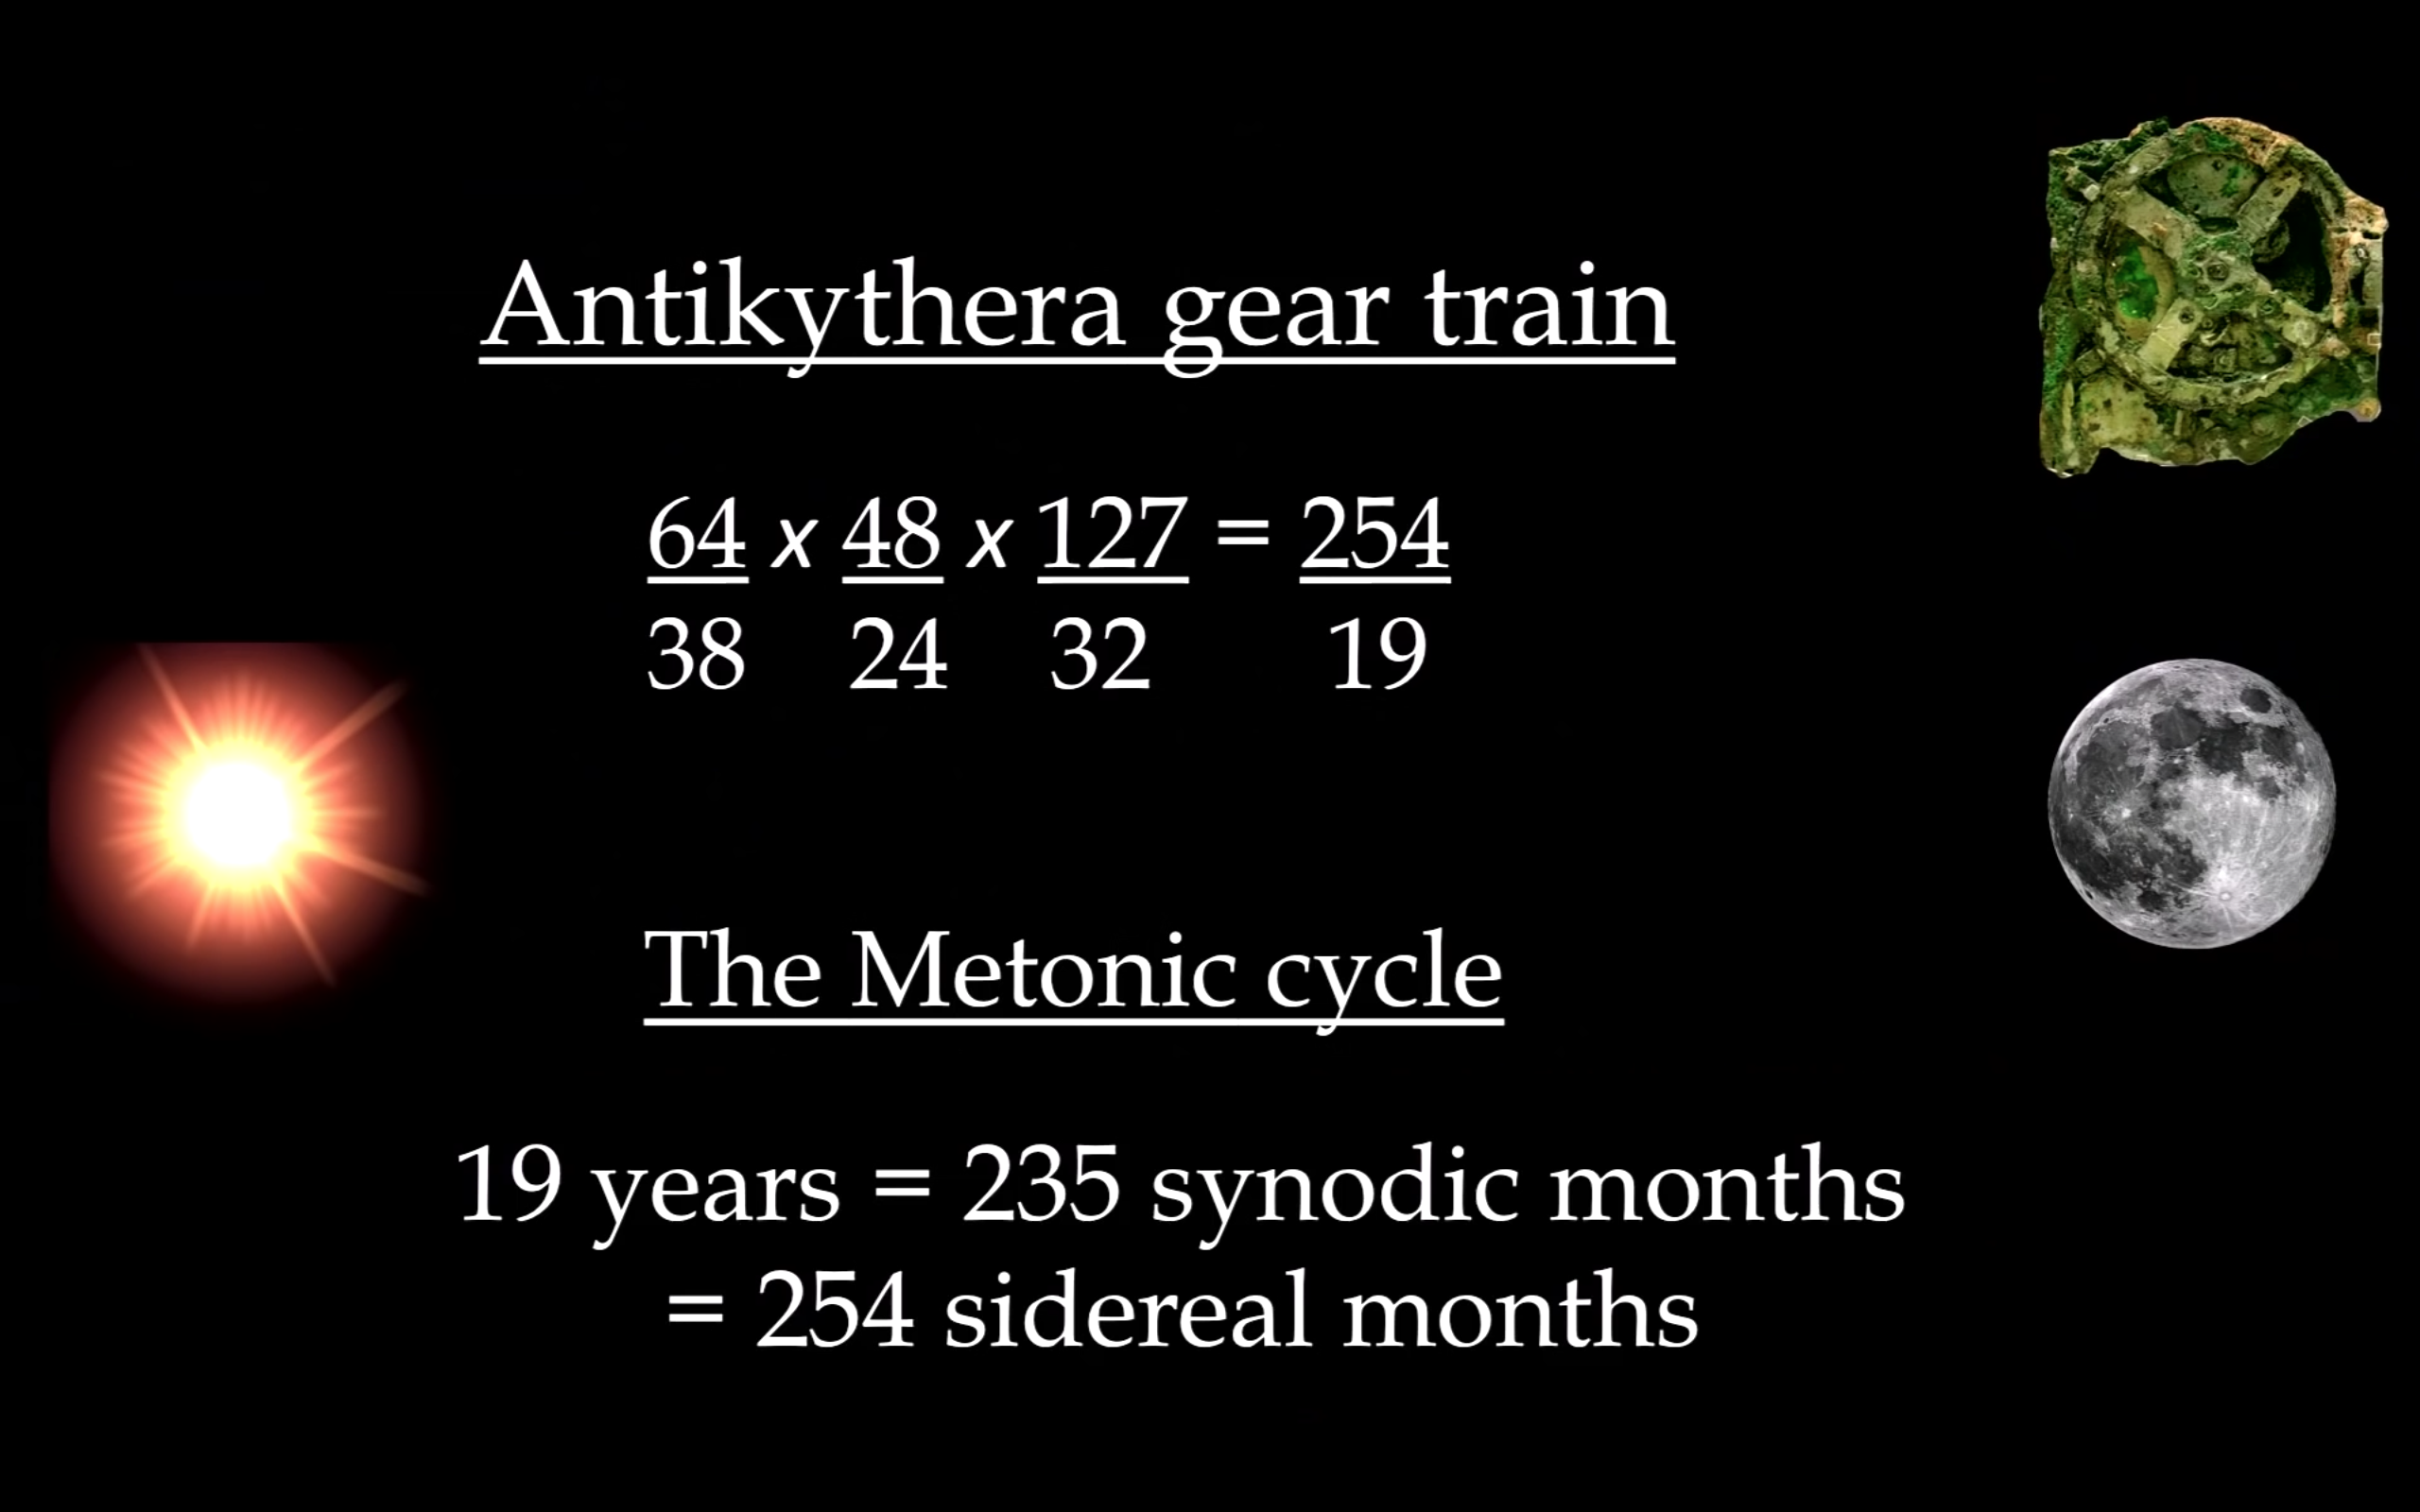
\includegraphics[scale=0.20,cfbox=red] {images/price_gear_train.png}}
\caption{Metonic Gear Train Ratios and the Metonic Cycle}
\label{fig:metonic_gear_ratios}
\end{figure}


\bigskip
\section{Putting It All Together}
The Antikythera Mechanism is thought to have been operated by a knob or crank on the side of the device. This knob (or crank) was connected
to a crown gear that meshed with b1, the main drive gear. b1 is the large, four spoked gear seen in Fragment A (see Figure \ref{fig:fragmentA}), 
and one revolution of b1 represents one year\footnote{For this reason b1 is sometimes called the "solar gear" \cite{pin_and_slot_device}.}. Since 
b2 is planted on b1 to form a compound gear (b1 and b2 are connected to the same axle; see Figures  \ref{fig:sectional_gearing} and \ref{fig:fragmentA}), 
one revolution of b2 also represents one year. 


\bigskip
\begin{figure}[H]
\center{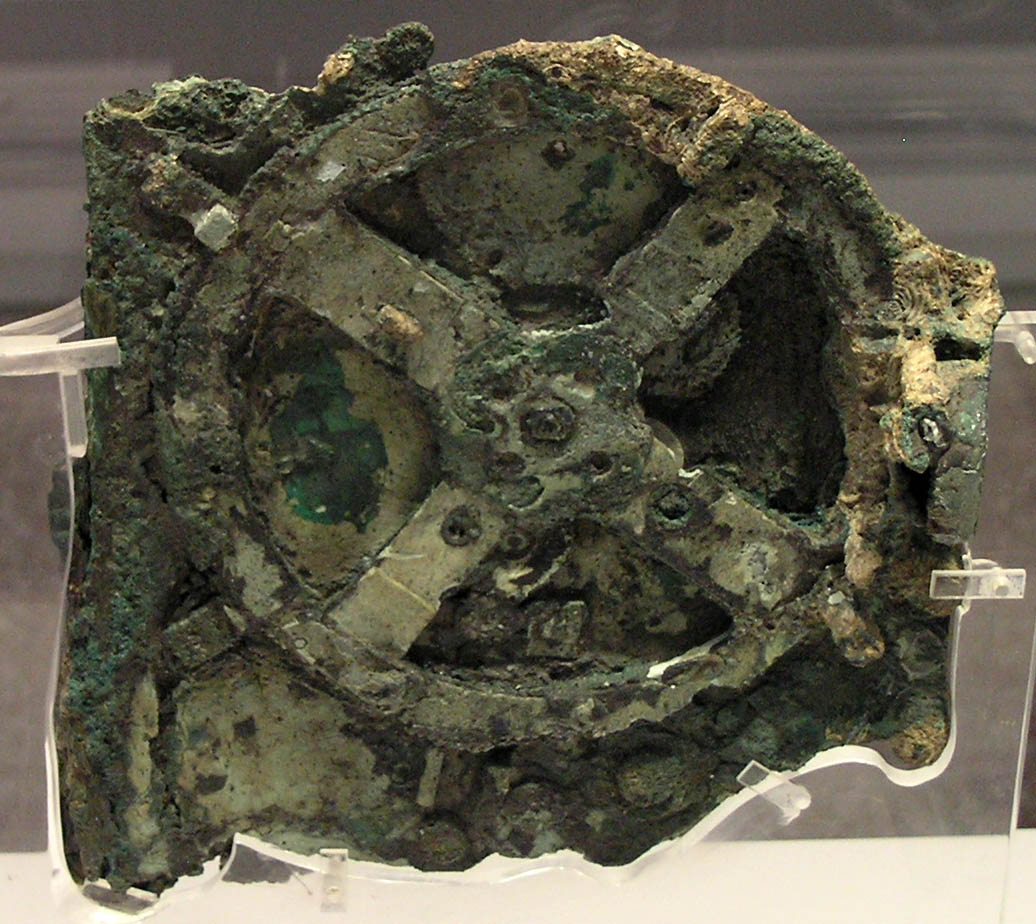
\includegraphics[scale=0.20,cfbox=red] {images/fragmentA.jpg}}
\caption{Fragment A of the Antikythera Mechanism \cite{wiki:fragmentA}}
\label{fig:fragmentA}
\end{figure}

\bigskip
\noindent
This configuration of gears means that one revolution of b2 (or b1) moves the Metonic pointer by one nineteenth of the Metonic Cycle, 
or 13.36842 sidereal months. Thus 19 revolutions of the main drive gear results in one revolution of the Metonic pointer or one Metonic Cycle, 
just as required.

\bigskip
\noindent
Unfortunately Price was wrong. He incorrectly thought that the output of his Metonic Cycle gear train, at gear e2,  went directly to the Zodiac dial 
on the front of the Mechanism that Albert Rehm \cite{wiki:rehm} had proposed to show the average position of the Moon in the Zodiac. What this
gear train actually does is to calculate the mean sidereal month which is used to drive the 50 tooth gear e5, which is the input to 
the pin-and-slot device.

\section{Michael Wright's Scheme For Turning The Metonic Pointer}
In Price's model the Metonic Cycle gear train output directly to a pointer on the proposed Zodiac dial on the front of the Mechanism. Michael Wright suggested 
a different scheme for the Metonic dial and pointer \cite{Wright2005a}. Wright noted Price's comment that the back upper dial, the Metonic 
dial, might be a five turn dial since  one Metonic cycle equals 235 synodic months which equals $5 \times 47 \text{ lunar months}$ \cite{gears_from_the_greeks}.
As a result Wright proposed that the Metonic dial was a five turn spiral dial in which each revolution represented 47 lunar months and  proposed the following 
gearing scheme to move the Metonic pointer on this five turn dial:

\bigskip
\bigskip
\begin{minipage}[c]{0.45\textwidth}
  \begin{itemize}
      \item l1: 38 teeth
      \item b2: 64 teeth
      \item l2: 53 teeth
      \item m1: 96 teeth
      \item m2: 15 teeth
      \item n1: 53 teeth
  \end{itemize}
\end{minipage}
\hfill
\begin{minipage}[c]{0.60\textwidth}
  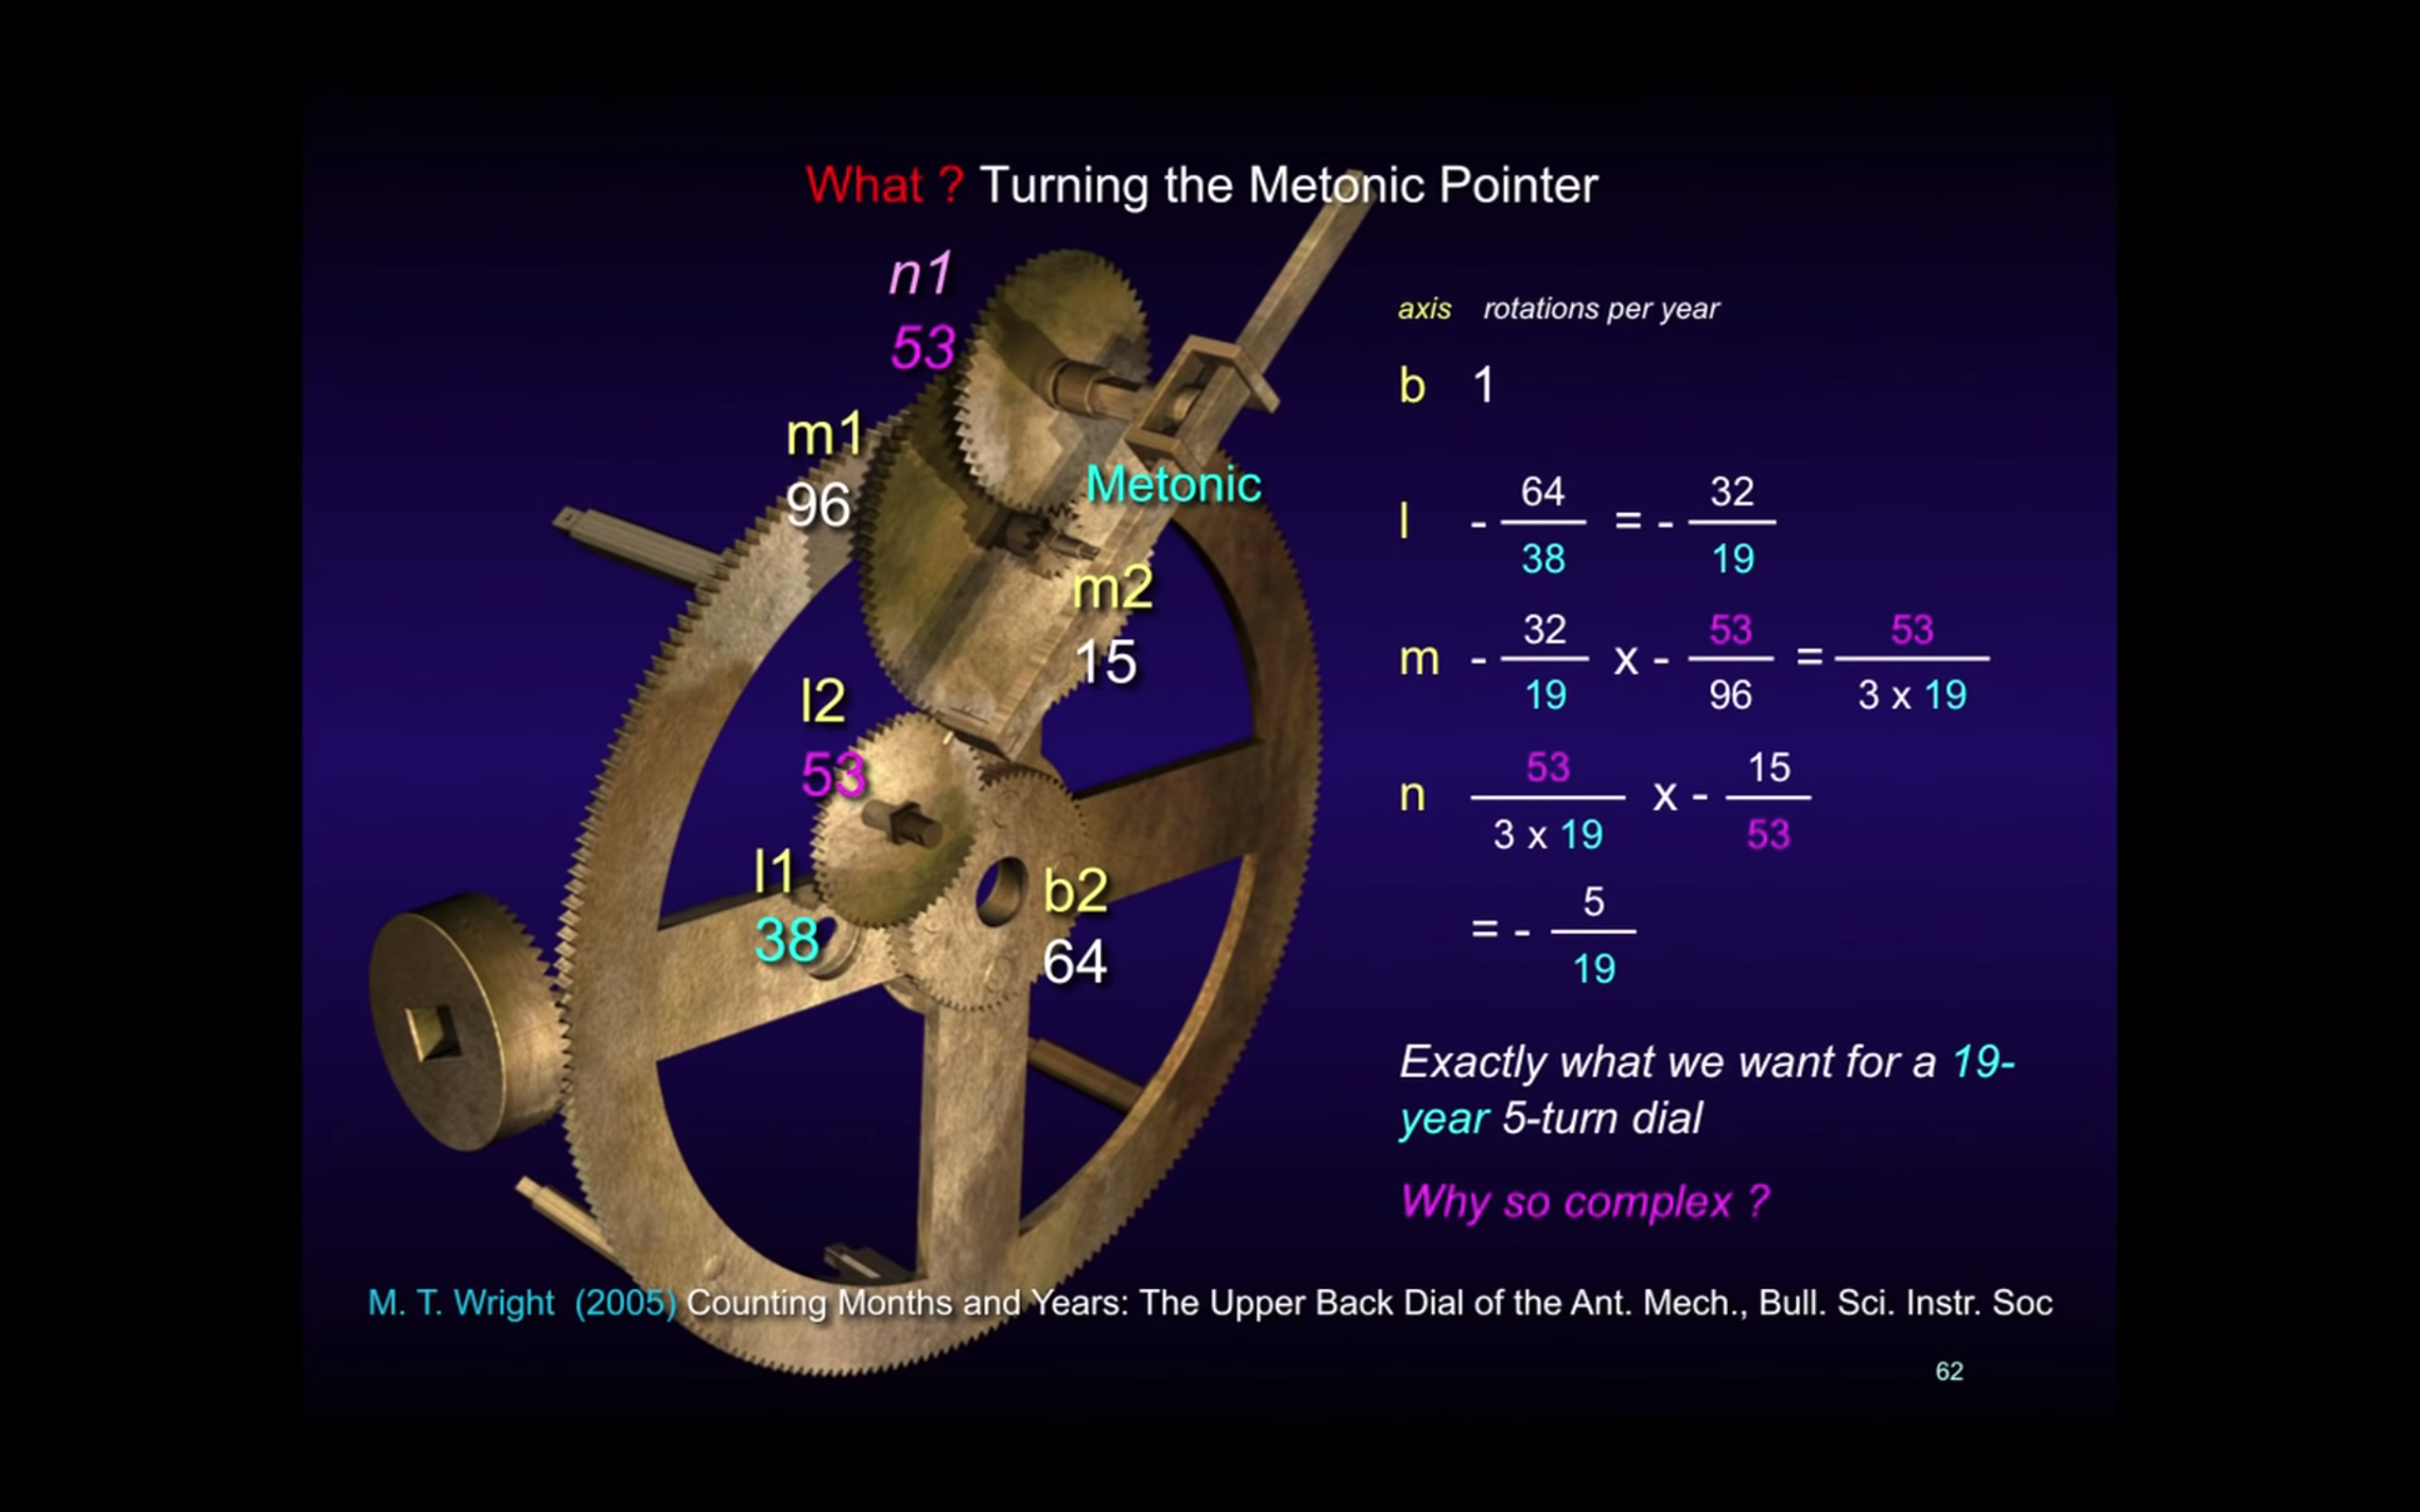
\includegraphics[width=\textwidth,cfbox=red]{images/turning_the_metonic_pointer_wright.png}
  \captionof{figure}{Wright's Metonic Gear Train \cite{youtube:freeth2021}}
\end{minipage}

\bigskip
\bigskip
\noindent
Wright's  gear ratios work out like this:

\bigskip
\begin{equation*}
\begin{array}{lllll}
- \frac{\text{b2}}{\text{l1}} &= - \frac{64}{38} = - \frac{32}{19}                                                                                                                                                              \\ \\
-\frac{\text{b2}}{\text{l1}} \times -\frac{\text{l2}}{\text{m1}} &= - \frac{64}{38} \times - \frac{53}{96} = - \frac{32}{19} \times - \frac{53}{96} = \frac{53}{3 \times 19}  \\ \\
- \frac{\text{b2}}{\text{l1}} \times -\frac{\text{l2}}{\text{m1}} \times - \frac{\text{m2}}{\text{n1}} &= - \frac{64}{38} \times - \frac{53}{96} \times - \frac{15}{53} 
=  -\frac{32}{19} \times - \frac{53}{3 \times 32} \times - \frac{3 \times 5}{53} = - \frac{5}{19}
\end{array}
\end{equation*}

\bigskip
\bigskip
\noindent
So one revolution of the main drive gear (b1) moves Wright's Metonic pointer by $\frac{5}{19} \approx 0.2632$, and nineteen revolutions of b1 (one Metonic Cycle) results in five
revolutions of Wright's Metonic pointer, consistent with Wright's five turn spiral Metonic dial model.


\bigskip
\noindent
BTW, note that the two 53 tooth gears l2 and n1 cancel in this gear train, so why are they there? 
Part of the answer is to drive the Saros eclipse prediction dial \cite{pmid25075747}, a subject for another note. 
However,  for reference: one Saros Cycle after an eclipse the Sun, Earth, and Moon return to approximately the same 
relative geometry (close to a straight line) and a nearly identical eclipse will occur in what is referred to as an eclipse 
cycle \cite{wiki:saros}. 

\bigskip
\noindent
It turns out that the Saros Cycle is a remarkable chance resonance between three of the orbital cycles of the moon: the synodic, draconic and anomalistic 
lunar cycles.

\begin{flushleft}
\begin{tabular}{@{}l@{\ }l@{\qquad}l}
  One Saros Cycle
  & = 223 synodic months                                                                                                \\
  & $\approx$ 242 draconic months                           &\# 241.999 draconic months       \\
  & $\approx$ 239 anomalistic months                       & \# 238.992 anomalistic months \\
  & $\approx$ 19 eclipse years (38 eclipse seasons) & \# 18.999 eclipse years             \\
  & = 6,585.321347 solar days                                                                                         \\
  & = 18.029  tropical years            
\end{tabular}
\end{flushleft}

\bigskip
\section*{Acknowledgements}

Thanks to Lars-Johan Liman for all of his help and LaTeX expertise. Thanks also to Dave Neary and Marshall Eubanks for their formatting suggestions.

%\newpage
\bibliographystyle{plain}
\bibliography{/Users/dmm/papers/bib/astronomy}
\end{document} 
